% 20 / 02 /2009 v1.00c TKZdoc-tab-tv
\section{Creating a table of variations in one step: \addbs{tkzTab}}
\subsection{Definition}
\begin{NewMacroBox}{tkzTab}%
{\oarg{local options}\var{list1}\var{list2}\var{list3}\var{list4}}

\medskip
\begin{tabular}{lllc}
\toprule
\texttt{arguments}   & \texttt{default}    & \texttt{definition}       \\
\midrule
\IargName{tkzTab}{list1}  & |no default|  & \var{e(1)/h(1),\dots,e(p)/h(p)} first column     \\
\IargName{tkzTab}{list2}  & |no default|  & \var{a(1),\dots,a(n)}    values of the first row  \\
\IargName{tkzTab}{list3}  & |no default|  & \var{s(1),\dots,s(2n-1)} symbols of the line of signs   \\
\IargName{tkzTab}{list4}  & |no default|  & \var{s(1)/eg(1)/ed(1),\dots,s($q$)/eg($q$)/ed($q$)} variations     \\
\bottomrule
\end{tabular}

\medskip
\noindent\emph{The macro \emph{\tkzcname{tkzTab}} is a shortcut for \tkzcname{tkzTabInit} followed by \tkzcname{tkzTabLine} and \tkzcname{tkzTabVar}. Its \tkzname{options} are the same as those of \tkzcname{tkzTabInit}. It only makes tables with three rows: the variable, the sign of the derivative and the variations of the function.}
\end{NewMacroBox}

\medskip

\begin{tkzexample}[code only]
 \tkzTab{ e(1) / h(1) ,
             ... ,
          e(p) / h(p)}
        { v(1), ... ,v(n) }
        { a(1),...,a(2n-1)}
        { s(1) / eg(1) / ed(1), ... ,s(n) / eg(n) / ed(n)}
\end{tkzexample}

\subsection{Example 1}

Study of the function $f~:~ x \longmapsto x^2$ on $[-5, 7]$

\begin{tkzexample}[vbox,small]
\begin{tikzpicture}
\tkzTab[lgt=3,espcl=5]{ $x$                    / 1,
                        $f'(x)$                / 1,
                        Variations of \\$f$ / 2}
                      { $-5$ , $0$ ,$7$}
                      { ,-,z,+,}
                      { +/$25$  , -/$0$  , +/ $49$}%
\end{tikzpicture}
\end{tkzexample}

\subsection{Example 2}
Study of the function $f~:~ x \longmapsto x \ln x $ on $(0, +\infty)$

\begin{tkzexample}[vbox,small]
 \begin{tikzpicture}
 \tkzTab[espcl=5,lgt=3]{$x$ / 1, Sign of \\$\ln x +1$ / 1.5,%
   Variations of \\$f$ / 3}%
   {$0$ ,$1/\E$ , $+\infty$}{d,-,z,+,}
   {D+/ $0$,%
    -/ \colorbox{black}{\textcolor{white}{$\dfrac{-1}{e}$}}  ,%
    +/ $+\infty$ }%
\end{tikzpicture}
\end{tkzexample}

\subsection{Example 3}
 Study of the function $f~:~ x \longmapsto \sqrt{x^2-1}$ on $(-\infty, -1] \cup [1, +\infty)$

\begin{tkzexample}[vbox,small]
\begin{tikzpicture}
  \tkzTab{ $x$ / 1, $f'(x)$ / 1, $f$ / 2}%
         { $-\infty$, $-1$ ,$1$, $+\infty$}
         { ,-,d,h,d,+, }
         { +/$+\infty$  , -H/$0$, -/$0$  , +/ $+\infty$  }%
\end{tikzpicture}
\end{tkzexample}

\subsection{Example 4}
 Study of the function $f~:~ t \longmapsto \frac{t^2}{t^2-1}$ on $[0, +\infty)$

\begin{tkzexample}[vbox,small]
\begin{tikzpicture}
  \tkzTab{ $t$ / 1, Sign of\\ $f'(t)$ / 2, Variations of \\$f$ / 2}%
         { $0$, $1$, $+\infty$}
         { z , - , d , - , }
         { +/$0$  , -D+/$-\infty$/$+\infty$, -/ $1$  }%
\end{tikzpicture}
\end{tkzexample}
\endinput
